\section{Graph $\theta$-Joins}\label{sec:grajoindef}
At the time of writing, the only field where graph joins where effectively
discussed is Discrete Mathematics. In this field such operations are defined
over either on finite graphs or on finite graphs with cycles, and are named
\textit{graph products} \cite{Hammack}. As the name suggests, every graph product of two graphs,
e.g. $G_1=(V_1,E_1)$ and $G_2=(V_2,E_2)$, produces a graph whose vertex set
is defined as $V_1\times V_2$, while the edge set changes accordingly to the
different graph product definition. Consequently the Kroneker Graph Product
\cite{Weichsel} is defined as follows:
\[G_1\times G_2=(V_1\times V_2, \Set{((g,h),(g',h'))\in V_1\times V_2|(g,g')\in E_1,(h,h')\in E_2})\]
while the \textit{cartesian graph product} \cite{ImrichP07} is defined as follows:
\[G_1\square G_2=(V_1\times V_2,\Set{((g,h),(g',h'))\in V_1\times V_2|(g=g',(h,h')\in E_2) \vee  (h=h', (g,g')\in E_1)})\]
Please observe that this definition creates a new vertex which is a pair of
vertices: hereby such operation is defined differently from the relational
algebra's cartesian product, where the two vertices are merged. As a consequence,
such graph products admit commutativity and associativity properties only up to
graph isomorphism. Other graph products are \textit{lexicographic product}
and \textit{strong product} \cite{Hammack,ProductGraphs}. Recently, a Kronecker Product for edge uncertainty was also provided \cite{Zhao17RH}, even though no information on how to combine the data associated to either vertices or edges was provided.

Consequently, even our graph join is based on
the combination of vertices and  edges: $G_a\bowtie_\theta^{\textup{\textbf{es}}}G_b$
expresses the join of graph $G_a$ with $G_b$ where
\begin{enumerate*}[label=\textit{(\roman*)}]
	\item we first use a relational $\theta$-join among the vertices,
	and then \item we combine the edges using an appropriate user-determined
	edge semantics, \textbf{es}\index{semantics!edge (graph join)}.
\end{enumerate*}
This  modularity is similar to
the operators previously described in graph theory literature, where instead of a join between vertices they have a
cross product, and different semantics are expressed as different
graph products.
We now provide the graph join definition:

\begin{definition}[Graph $\theta$-Join]\label{def:join}
	\label{def:graphjoin} \index{product, $\otimes_\theta$!for property graphs!join}\index{$\bowtie$!property graphs|see {product $\otimes_\theta$}}
	Given two graphs $G_a=(V,E,A_v,A_e)$ and $G_b=(V',E',A_v',A_e')$, a \textbf{graph
		$\theta$-join} is defined as follows:
	\begin{equation*}
	G_a\bowtie_\theta^{\textbf{\textup{es}}} G_b=(V\bowtie_\theta V',E_{\textup{\textbf{es}}},A_v\cup A_v',A_e\cup A_e')
	\end{equation*}
	where $\theta$ is a binary predicate over the vertices and $\bowtie_\theta$ the $\theta$-join (Definition \ref{def:thetajoin}) among the vertices, and
	$E_{\textup{\textbf{es}}}$ is a subset of all the possible edges linking the vertices in $V\bowtie_\theta V'$ expressed
	with the \textup{\textbf{es}} semantics.
\end{definition}
Given that graph join
returns a property graph like the graphs in input, property graphs are
closed under the graph join operator via the definition of $\oplus$ for the multiset
$\theta$-join. Moreover, this allows a first step towards the edge result combination as required by some data integration scenarios. For example,
The result of the join between two graphs, ResearchGate (Figure \ref{g:en}) and References (Figure \ref{g:dep}), produces the same
set of vertices regardless of the edge semantics of choice. On the other hand, edges among the resulting vertices change according to the edge semantics. In the first one (Figure \ref{g:conjo}) we  combine edges appearing in both graphs
and linking vertices that appear combined in the resulting graph. We have a \textbf{Conjunctive Join}, that in graph theory is known as \textit{Kronecker graph product} \cite{Weichsel,Hammack}.
In this case  $E_{\textup{\textbf{es}}}$ is defined with the ``$\wedge$'' \textbf{es} semantics as an edge join
$E_{\wedge}=E\bowtie_{\Theta_\wedge}E'$, where the ${\Theta_\wedge}$ predicate is the following one:
\begin{equation}
\label{eq:conj}
\Theta_\wedge(e_h,e_k')=(e_h\in E\wedge e_k'\in E') \wedge \lambda(e_h\oplus e_k')\in (V\bowtie_\theta V')^2
\end{equation}



We can also define a \textbf{disjunctive} semantics (Figure \ref{g:depjo}), having ``$\vee$'' as \textbf{es}.
In this case we want edges appearing either in the first or in the second operand.
This means that two vertices, $u_h\oplus u'_h$ and $v_k\oplus v'_k$, {{could}} have a resulting
edge
%\footnote{$\lambda(e\oplus e')=\lambda(e)\oplus\lambda(e')=(u,u')\oplus (v,v')=(u\oplus v, u'\oplus v')$}
$e_i\oplus \varepsilon'_j$
even if only $\lambda(e_i)=(u_h,v_k)$ appears in the first operand\footnote{The statement addressing the edges in the second operand that do not bond with the ones in the other graph is expressed as follows: $\forall e'\in E'. \neg\Theta_\wedge(e_i,e')$}
and $\varepsilon'$ is a ``fresh'' empty edge $\lambda(\varepsilon'_j)=(u'_h,v'_k)$ not
appearing in $G_b$ such that $\lambda(e_a\oplus \varepsilon'_b)=(u_h\oplus u'_h,v_k\oplus v'_k)$.
%\footnote{$\forall e'\in E',\neg\Theta(e,e')$}. In order to do so we have to define
%In order to do so we have to define
%$e'$ as a new empty tuple $\varepsilon_i$ belonging to no graph such that
%\footnote{We could consider the following definition as a full outer join betweenl
%	$E$ and $E'$.}
%$\lambda(\varepsilon_i,0)=(v,v')$.
Consequently the disjunctive join can be represented as a \textit{full outer join}, where the
edges either match in the conjunctive semantics, or appear in the two distinct graph operands:


\begin{align*}
E_{\vee}&=E\fullouterjoin_{\Theta_\wedge}E'&&\cup\{(e_i\oplus\varepsilon_j)|\varepsilon_j,\,\left(\forall e'\in E'. \neg\Theta_\wedge(e_i,e')\right), \ell_e(\varepsilon_j)=\emptyset,\;\lambda(e_i)\oplus (v,v')\in (V\bowtie_\theta V')^2  \}\\
& && \cup\{(\varepsilon_i\oplus e_j)|\varepsilon_i,\,\left(\forall e\in E. \neg\Theta_\wedge(e,e_j)\right), \ell_e(\varepsilon_i)=\emptyset,\;(u,u')\oplus \lambda(e_j)\in (V\bowtie_\theta V')^2  \}\quad \\
&=  E\;\fullouterjoin_{\Theta_\wedge}\;E'
\end{align*}

\subsection{Graph Join properties}
With this section we want to discuss some properties of graph joins that allow to analyse their scalability with respect to the generalization of such joins to multiple graphs.
We could first check that the proposed graph $\theta$-join is closed under composition:
it takes two (property) graphs and returns a property graph as an output by construction.
We discuss the commutativity and the associativity for graph joins in each semantics.
\begin{lemma}[Join Commutativity]
	Given two graphs $G$ and $G'$ from the same graph database $\mathcal{D}$ and a symmetric binary predicate
	$\theta$, then we have $G\bowtie_\theta^\wedge G' \equiv G'\bowtie_{\theta^{-1}}^\wedge G$ for the conjunctive
	semantics and $G\bowtie_\theta^\vee G' \equiv G'\bowtie_{\theta^{-1}}^\vee G$ for the disjunctive one.
\end{lemma}
\begin{proof}
We first choose $\theta^{-1}$ as the inverse predicate of $\theta$, such that $\theta^{-1}(b,a)\Leftrightarrow \theta(a,b)$. For the conjunctive semantics, we have that $G\bowtie_\theta^\wedge G'$ is:
	\[(V\bowtie_\theta V',E\bowtie_{\Theta_\wedge}E', A_v\cup A_v',A_e\cup A_e',\mathcal{V}_v\cup \mathcal{V}_v',\mathcal{V}_e\cup \mathcal{V}_e')\]
	Since we have that $V\bowtie_\theta V'=V'\bowtie_{\theta^{-1}} V$ and
	$E\bowtie_{\Theta_\wedge}E'=E'\bowtie_{\Theta_\wedge}E$, then we have that
	the graph join is equivalent to $G'\bowtie_{\theta^{-1}}^\wedge G$.

	This is proved because the relational join between vertices and edges is  a commutative operator
	\cite{Rolleke94equivalencesof}, and predicate $\Theta_\wedge$  is symmetric
	when either $E$ and $E'$ or $E'$ and $E$ are joined. A similar proof could be carried out for
	the disjunctive semantics, since it is in the form:

	\begin{align*}
	\label{eq:disj}
	&E\fullouterjoin_{\Theta_\wedge}E'&\cup\{(e_i\oplus\varepsilon_j)|\varepsilon_j,\,\left(\forall e'\in E'. \neg\Theta_\wedge(e_i,e')\right), \ell_e(\varepsilon_j)=\emptyset,\;\lambda(e_i)\oplus (v,v')\in (V\bowtie_\theta V')^2  \}\\
	& & \cup\{(\varepsilon_i\oplus e_j)|\varepsilon_i,\,\left(\forall e\in E. \neg\Theta_\wedge(e,e_j)\right), \ell_e(\varepsilon_i)=\emptyset,\;(u,u')\oplus \lambda(e_j)\in (V\bowtie_\theta V')^2  \}\quad \\
	&= E'\fullouterjoin_{\Theta_\wedge}E& \cup\{(e_j\oplus \varepsilon_i)|\varepsilon_i,\,\left(\forall e\in E. \neg\Theta_\wedge(e,e_j)\right), \ell_e(\varepsilon_i)=\emptyset,\;(u',u)\oplus \lambda(e_j)\in (V'\bowtie_\theta V)^2  \}\quad \\
	& & \{(\varepsilon_j\oplus e_i)|\varepsilon_j,\,\left(\forall e'\in E'. \neg\Theta_\wedge(e_i,e')\right), \ell_e(\varepsilon_j)=\emptyset,\;\lambda(e_i)\oplus (v',v)\in (V'\bowtie_\theta V)^2  \}\\
	&
	\end{align*}

%\[E\bowtie_{\Theta_\wedge}E'\cup \{(e_j\oplus \varepsilon_i)|\dots\}\cup \{(\varepsilon_i\oplus e_j')|\dots\}=E'\bowtie_{\Theta_\wedge}E\cup \{( e_j'\oplus \varepsilon_i)|\dots\}\cup  \{( \varepsilon_i\oplus e_j)|\dots\}\]
This equation is true because the relational join is symmetric
	as the set union and the $\oplus$ operator with the null tuple $\varepsilon_i$.
\end{proof}

The following corollary strengthens the previous result: it shows that join commutativity implies
having two resulting graphs where both vertices and edges have the same labels, and the same edges
link the same vertices.

\begin{corollary}[Commutativity for $\lambda$, $\ell_v$ and $\ell_e$]\label{coroll:Comm}
	For each vertex $v_i\oplus v_j'$ from the vertex set $V\bowtie_\theta V'$ from
	$G\bowtie_\theta^\wedge G'$ and the corresponding equivalent vertex $v_j'\oplus v_i$ in $V'\bowtie_\theta V$ from
	$G'\bowtie_\theta^\wedge G$ ($v_i\oplus v_j'=v_j'\oplus v_i$), we have that both vertices have the same label set.

	For the conjunctive semantics, for each edge $e_h\oplus e_k'$ from the edge set $E\bowtie_{\Theta_\wedge} E'$ from
	$G\bowtie_\theta^\wedge G'$ and the corresponding equivalent edge $e_k'\oplus e_h$ in $E'\bowtie_{\Theta_\wedge} E$ from
	$G'\bowtie_\theta^\wedge G$ ($e_h\oplus e_k'=e_k'\oplus e_h$), we have that both edges have the same label set and link
	the same equivalent vertices. This statement also applies for the disjunctive semantics.
\end{corollary}
\begin{proof}
	This corollary is proved by the linearity of $\oplus$. Regarding the vertex labelling, we have that the labelling provided by the result of the two commutated joins is the same by the commutativity of the set union operator:
	\[\begin{split}
	\ell_v(u_i\oplus u_j')&=\ell_v(u_i)\oplus \ell_v(u_j')=\ell_v(u_i)\cup\ell_v(u_j')=\\
	&=\ell_v(u_j')\cup\ell_v(u_i)=\ell_v(u_j')\oplus\ell_v(u_i)=\\
	&=\ell_v(u_j'\oplus u_i)
	\end{split}
	\]

	Regarding the conjunctive semantics, the proof of $\ell_e(e_h\oplus e_k')=\ell_e(e_k'\oplus e_h)$ is similar, by using the set union's commutativity. We  prove that equivalent edges link equivalent vertices:
	\[\begin{split}
	\lambda_{E_\wedge}(e_h\oplus e_k')&=\lambda_E(e_h)\oplus\lambda_{E'}(e_k')=(u_i,v_j)\oplus (u_l',v_m')=\\
	&=(u_i\oplus u_l',v_j\oplus v_m')=(u_l'\oplus u_i,v_m'\oplus v_j)
	\end{split}  \]
	\[\lambda_{E_\wedge}(e_k'\oplus e_h)=\lambda_{E'}(e_k')\oplus\lambda_{E'}(e_k')=(u_l'\oplus u_i,v_m'\oplus v_j)  \]
	The proofs for the disjunctive semantics are the same.
\end{proof}

Since the relational algebra $\theta$-join operator satisfies associativity \cite{Rolleke94equivalencesof}, we could carry out a similar
proof for join associativity:

\begin{lemma}[Join Associativity]
	Given three graphs $G$, $G'$ and $G''$ from the same graph database $\mathcal{D}$ and a symmetric binary predicate
	$\theta$, then we have $G\bowtie_{\theta_1\wedge\theta_\alpha}^\wedge (G'\bowtie_{\theta_2}^\wedge G'') = (G\bowtie_{\theta_1}^\wedge G')\bowtie_{\theta_\alpha\wedge \theta_2}^\wedge G''$ for the conjunctive
	semantics and $G\bowtie_{\theta_1\wedge\theta_\alpha}^\vee (G'\bowtie_{\theta_2}^\vee G'') = (G\bowtie_{\theta_1}^\vee G')\bowtie_{\theta_\alpha\wedge\theta_2}^\vee G''$ for the disjunctive one.
\end{lemma}
\begin{proof}
Since we have that the usual $\theta$-relational joins are associative as outlined by the following equivalence:
\[(A\bowtie_{\theta_1}B)\bowtie_{\theta_\alpha\wedge \theta_2}C =A\bowtie_{\theta_1\wedge\theta_\alpha}(B\bowtie_{\theta_2}C)\]
then, we have that the relational $\theta$-joins among the edges are associative too, as well as the theta joins among the edges. Hereby, the join between the graphs is associative. 
\end{proof}

Similarly to the graph join's commutativity, we can strengthen the result for the join associativity with the following corollary:

\begin{corollary}[Associativity for $\lambda$, $\ell_v$ and $\ell_e$]\label{coroll:Comm}
	For each vertex $v_i\oplus (v_j' \oplus v_k'')$ from the vertex set $V\bowtie_{\theta_1\wedge\theta_\alpha}^\wedge (V'\bowtie_{\theta_2}^\wedge V'')$ from
	$G\bowtie_{\theta_1\wedge\theta_\alpha}^\wedge (G'\bowtie_{\theta_2}^\wedge G'')$ and the corresponding equivalent vertex $(v_i\oplus v_j')\oplus v_k''$ in $V'\bowtie_\theta V$ from
	$(G\bowtie_{\theta_1}^\wedge G')\bowtie_{\theta_\alpha\wedge \theta_2}^\wedge G''$ ($v_i\oplus (v_j'\oplus v_k'')=(v_i\oplus v_j')\oplus v_k''$), we have that both vertices have the same label set.

	For the conjunctive semantics, for each edge $e_h\oplus (e_k'\oplus e_t'')$ from the edge set $E\bowtie_{\Theta_\wedge} (E'\bowtie_{\Theta_\wedge}E'')$ from
	$G\bowtie_{\theta_1\wedge\theta_\alpha}^\wedge (G'\bowtie_{\theta_2}^\wedge G'')$ and the corresponding equivalent edge $(e_h\oplus e_k')\oplus e_t''$  from
	$ (G\bowtie_{\theta_1}^\wedge G')\bowtie_{\theta_\alpha\wedge \theta_2}^\wedge G''$, we have that both edges have the same label set and link
	the same equivalent vertices. This statement also applies for the disjunctive semantics.
\end{corollary}
\begin{proof}
	This corollary is proved by the linearity of $\oplus$. Regarding the vertex labelling, we have that the labelling provided by the result of the two commutated joins is the same by the associativity of the set union operator:
	\[\begin{split}
	\ell_v(u_i\oplus (u_j'\oplus u_k''))&=\ell_v(u_i)\oplus \ell_v(u_j'\oplus u_k'')=\ell_v(u_i)\cup\ell_v(u_j')\cup\ell_v(u_k'')=\\
	&=\ell_v(u_i\oplus u_j')\oplus\ell_v(u_k'')=\ell_v((u_i\oplus u_j')\oplus u_k'')
	\end{split}
	\]

	Regarding the conjunctive semantics, the proof of $e_h\oplus (e_k'\oplus e_t'')=(e_h\oplus e_k')\oplus e_t''$ is similar, by using the set union's associativity. We  prove that equivalent edges link equivalent vertices:
	\[\begin{split}
	\lambda_{E_\wedge}((e_h\oplus e_k')\oplus e_t'')&=\lambda_E(e_h\oplus e_k')\oplus\lambda_{E'}(e_t'')=(u_i\oplus u_l',v_j\oplus v_m')\oplus(u_n'',u_p'')=\\
	&=(u_i\oplus u_l'\oplus u_n'',v_j\oplus v_m'\oplus u_p'') = \lambda_{E_\wedge}(e_h\oplus (e_k'\oplus e_t''))
	\end{split}  \]
	The proofs for the disjunctive semantics are the same.
\end{proof}

These properties for the graph joins prepare to a scalable implementation of multi-way graph joins: we could start to perform such joins from the smallest graph up to the greatest graph, such that the number of bucket comparisons is reduced.


\section{Graph Conjunctive Equi-Joins}
In the present section we're going to first describe the graph equi-join for $\theta$ conjunctive equijoins, and then introduce the secondary memory graph representation used by the presented algorithm (Section \ref{sec:algo}). In Section \ref{sub:results} we're going to compare our proposed algorithm (GCEA) to both graph database libraries (Section \vref{sec:qbench}), on top of which the same algorithm is implemented and evaluated, and graph query languages on top of specific graph databases (Section \vref{sec:qplan}), thus comparing the efficiency of our algorithm to their query plan evaluation.

\subsection{Algorithm and Data Structure}
\label{sec:algo}
\begin{algorithm}[!b]
	\caption{Graph Conjunctive EquiJoin Algorithm (GCEA)}\label{alg:cogrouped}
	{
		\begin{minipage}{\linewidth}
			\begin{algorithmic}[1]
				\Procedure{ConjunctiveJoin}{$G,G',\theta$}
				\State \textit{hashFunction} = generateHash($\theta$);
				\State \textit{omap}$_1$ = \textsc{OperandPartitioning}($G,$\textit{hashFunction})
				\State \textit{omap}$_2$ = \textsc{OperandPartitioning}($G',$\textit{hashFunction})
				\State $\overline{G}_1$ = \textsc{SerializeOperand}($G,$\textit{omap}$_1$)
				\State  $\overline{G}_2$ = \textsc{SerializeOperand}($G',$\textit{omap}$_2$)

				\Return{\textsc{PartitionHashJoin}($\overline{G}_1,\overline{G}_2,\theta$)}
				\EndProcedure

				\State



				\Procedure{SerializeOperand}{$G,$omap}:
				\State \textsc{File} \textit{VertexIndex} = \textsc{Open()};
				\State \textit{VertexVals}= \textsc{Open()}, \textit{HashOffset}= \textsc{Open()};
				\State \textbf{ulong} \textit{offset} = \textit{HashOffset} = 0;
				\For{\textbf{each} $h\in$\textsc{Keys}(omap)} \Comment{Ordered maps have ordered keys.}
				\State \textit{HashOffset}.\textsc{Write}(\{$h$,\textit{HashOffset}\});
				\For{\textbf{each} $id\in $omap[$h$]}
				\State $v$ = $G$.$V$[$id$];
				\State $v$.hash = $h$; $v$.offset = \textit{VertexVals};
				\State \textit{VertexIndex}.\textsc{Write}(\{$v$.id,\;$h$,\;\textit{offset}\});
				\State \textbf{ulong} offsetNext = \textit{VA}.\textsc{Write}(\textsc{serialize}(v));
				\State \textit{offset}\texttt{+=}offsetNext; \textit{HashOffset}\texttt{+=}offsetNext;
				\EndFor
				\EndFor
				\Return{(\textit{VertexIndex},\textit{VertexVals},\textit{HashOffset},\textit{G.}$A_v$,\textit{G.}$A_e$)}
				\EndProcedure


				\State


				\Procedure{PartitionHashJoin}{$G_1,G_2,\theta$}:
				\State $\theta'(u,u')$ := $\theta(u,v)\wedge (u\oplus u')(A_v)=u\wedge (u\oplus u')(A_v')=u'$;
				\State $\Theta'(e,e')$ := $(e\oplus e')(A_e)=e \wedge (e\oplus e')(A_e')=e'$
				\State $HI$ = \textsc{IntersectHashes}(\textit{HashOffset}$_1$,\textit{HashOffset}$_2$).\textsc{iterator}();
				\State \textsc{File} $AdjFile$ = \textsc{Open}();
				\While{$HI$.\textsc{hasNext}()}
				\State $h$ = $HI$.\textsc{next}();
				\For{\textbf{each} $u\in \textit{VertexVals}_1[h.\textup{offset}_1]$, $u'\in \textit{VertexVals}_2[h.\textup{offset}_2]$}
				\If{$\theta'(u,u')$}
				\State{\textit{AdjFile}}.\textsc{Write}(V=\{$u\oplus u'$\},)
				\State $HIout$ = \textsc{IntersectHashes}($out_{V}(u)$,$out_{V'}(u')$).\textsc{iterator}();\label{code:vintersection}
				\While{{$HIout$.\textsc{hasNext}()}}
				\State {$h_{out}$ = $HIout$.\textsc{next}();}\Comment{\textit{Offsets refer to the blocks for $u$ and $u'$ outgoing edges}}
				\For{\textbf{each edge} $e\in out_{V}(u)[h_{out}.\textup{offset}_1]$, $e'\in out_{V'}(u')[h_{out}.\textup{offset}_2]$ }
				\If{$\theta'(e.\textup{outv},e'.\textup{outv})$\textbf{ and }$\Theta'(e,e')$}
				\State \textit{AdjFile}.\textsc{Write}(E=\{$e\oplus e'$\})
				\EndIf
				\EndFor
				\EndWhile
				\EndIf
				\EndFor
				\EndWhile

				\EndProcedure
			\end{algorithmic}
		\end{minipage}}
	\end{algorithm}
	We now outline our algorithm, GCEA\index{algorithm!GCEA}, for $\theta$ equijoin predicates, involving an
equivalence between attributes or a conjunction of such equivalences. We also suppose that both graph operands are always stored within the same graph database, and that the query itself will be provided to be read inside the same database environment.
The query result
is read only as in other graph query languages (SPARQL, SQL for databases) and does not correspond to a ``materialized view''. Therefore, the result of the graph query itself can postpone the creation of a complete property graph output (that is, the complete attribute-value and label information for our graphs).

		The starting point of each data integration procedure is the identification of
		similar pieces of data occurring into the to-be-merged operands. In our case, the
	graph { {integration}} task starts from the identification of the to-be-joined vertices
		and, after that, we have to decide how to combine the outgoing edges. The most
		intuitive way to match similar data content is to use equivalence predicates.
		
		

		
		
	This specific predicate choice was driven by the fact that the most performant
	and implemented relational database join is the equi-join \cite{SchuhCD16}, and that the result of relational databases' queries already produces join indices \cite{dittrich} where only the left and right operand indices are kept in the final result, so that the relational tables' pieces of informations are kept in primary memory purely as indices. Please also note that not all the graph join's equijoin predicates may be optimized\footnote{Consider two relations $R(A_1,A_2)$ and $S(A_3,A_4)$ within the relational model; we want to $\theta$-join them using the following predicate:
	\[\theta(r,s)=r[A_1]-s[A_4]=r[A_2]\cdot s[A_3]\]
Since this predicate requires performing arithmetical operations between attributes appearing in distinct relations ($r[A_1]-s[A_4]$) which evaluation requires the computation of all the $R\times S$ tuples, such predicate cannot benefit from a preliminary hashing and bucketing step.} and consequently, in some cases we must undoubtedly pay the computational price of the cartesian product.
	Moreover, we provide an implementation for {conjunctive semantics}, since this task is more prone to be
	optimized than the disjunctive one. Algorithm \ref{alg:cogrouped} for GCEA
	consists in three parts: \begin{enumerate*}[label=\textit{(\roman*)}]
		\item vertex partitioning (bucketing) through an hashing function (\textsc{Operand\-Partitioning})
		\item graph serialization on secondary memory (\textsc{SerializeOperand}), and
		\item actual join algorithm over the  graphs' buckets (\textsc{Par\-ti\-tion\-HashJoin}).
	\end{enumerate*}
	Relational partition hash-join undergo the same phases, even if relational algorithms
	do not deal with outgoing edges (lines 31-35).
	We allow vertices with replicated values as in current graph databases
	implementations (such as Titan and Neo4J). Consequently, $id$s enumerate the vertices
	within a single graph.

	\begin{figure*}[!t]
		\centering
		\begin{minipage}[b]{.5\textwidth}
			\centering
			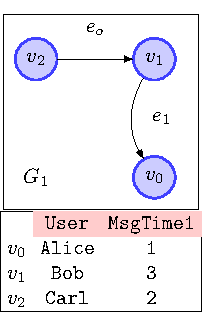
\includegraphics{fig/03joins/serialized_orig.pdf}
			\subcaption{$G_1$: an example property graph that is going to be serialized using our proposed indexing structure.}\label{fig:figjoing1bis}
		\end{minipage}
		\begin{minipage}[b]{\textwidth}
			\centering
			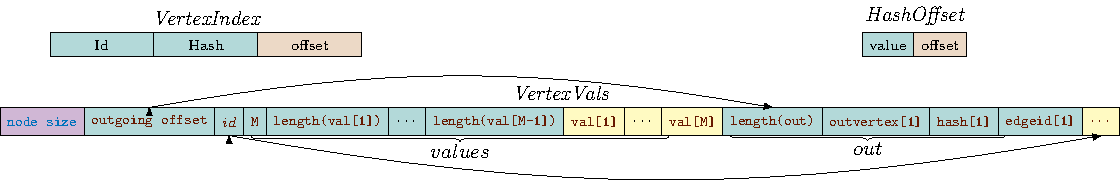
\includegraphics[width=\textwidth]{fig/03joins/serialized_structure2.pdf}
			\subcaption{Data structures used to implement the graph in secondary memory. Each data structure represents a different file.}\label{fig:graphstructure}
		\end{minipage}\\
			%\hspace*{-0.5cm}
		 \begin{minipage}[b]{\textwidth}
		 	\centering
		 	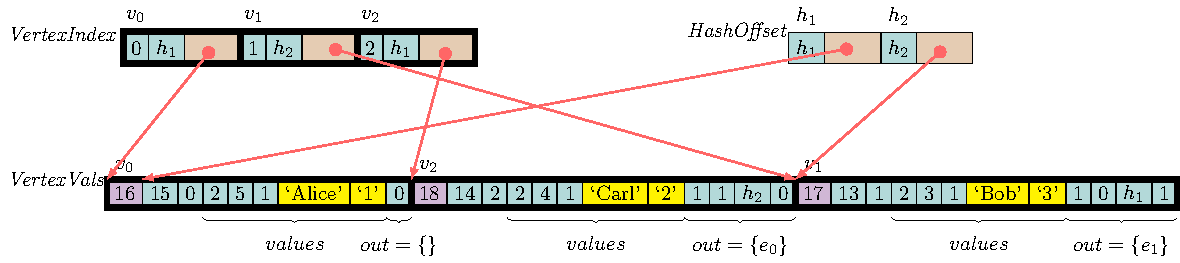
\includegraphics[width=\textwidth]{fig/03joins/serialized_ex2.pdf}
		 	\subcaption{Using the graph schema in Figure \ref{fig:graphstructure} for
		 		representing $G_1$ in secondary memory. $v_0$ and $v_2$ belong to a different bucket from $v_1$ only
		 		for illustrative purposes.}\label{fig:graphimplement}
		 \end{minipage}%
	 
	\begin{minipage}[b]{\textwidth}
		\centering
		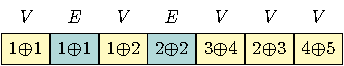
\includegraphics[width=.5\textwidth]{fig/03joins/02dlgorithm.pdf}
		\subcaption{Representing the serialization of the join ResearchGate$\Join^{\wedge}_{\texttt{Name}=\texttt{1Author}}$Reference depicted in Figure \vref{g:conjo}.}\label{fig:graphserres}
	\end{minipage}%
	
	
	\caption{\textit{Graph representation in secondary memory}.}
\end{figure*}
As a first step, the hashing function $h$ is inferred from $\theta$ (line 2): if $\theta(u,v)$ is a binary
predicate between distinct attributes from $u$ and $v$, then $h$ is defined as a linear combination of
hash functions over the attributes of either $u$ or $v$. When no $h$ {{could}} be inferred from $\theta$, then
$h$ is a constant function.

\textsc{OperandPartitioning} performs a vertex bucketing in main memory: its outcome
is an ordered map, where each vertex $v$ is stored in a collection $omap[h(v)]$, where $h$ is the aforementioned hashing function. For each operand $G_i$, the $omap_i$ construction  takes at most $\sum_{j=0}^{|\mathcal V(i)|}\log(j)$ time,
where $|\mathcal V(i)|$ is the multiset vertex size. Such time complexity
is bounded by $|\mathcal V(i)|\leq \sum_{j=0}^{|\mathcal V(i)|}\log(j)<|\mathcal V(i)|^2$ where $|\mathcal V(i)|\gg 1$.

\textsc{SerializeOperand} stores the operand in secondary memory: both buckets (line 12)
and vertices (line 14) are already sorted by hash value, and hence such data
structures are accessed linearly. Figure \ref{fig:graphimplement} depicts a serialized
representation of the graph in Figure \ref{fig:figjoing1bis}: all the labels and the edge values are not serialized but are still accessible through
the original graph $G$ via $id$. Moreover, such representation provides a adjacency list representation of graphs, that has been already proved to be graph traversal efficient, even in distributed computation contexts \cite{Labouseur2015}. Buckets are represented by \textit{HashOffset} providing both the bucket value
and the pointer to the first vertex of the bucket stored in \textit{VertexVals}.
\textit{VertexVals} stores vertices alongside with their adjacency list, where vertices are sorted by hash value
and are represented by \textit{id} and hash value.
\textit{VertexIndex} allows to find the vertices stored in \textit{VertexVals} in constant time:
each record  is ordered by vertex $id$, has a constant size
and contains the pointer to where the vertex data is stored in \textit{VertexVals}.
Even the outgoing edges are stored by the destination vertex's hash value.
Given $k_i$ the size of \textsc{Keys}(omap$_i$), this phase takes $3k_i+|G_i|$ time, where
$2k_i$ is the omap visit cost, $k_i$ is the omap serialization as \textit{HashOffset} and
$|G_i|$ is the time to serialize the graph as $VA_i$.


\begin{algorithm}[!b]
	\caption{Graph Disjunctive EquiJoin Algorithm: Join Phase}\label{alg:disjunctiveJOIN}

	\begin{adjustbox}{max width=\textwidth}
		\begin{minipage}{1.2\linewidth}
			\begin{algorithmic}[1]
				\Procedure{DisjunctiveEdges}{$G_1,G_2,\Braket{HI,\hbar,\Delta E_1,\Delta E_2,\textit{f}}$}:
					\State {$offsets:=$find($\hbar$,\;$HI$)}\label{line:intersectionwithfind}
					\If{$\hbar.\textup{offset}_1\neq$\texttt{NULL} \textbf{and} $offsets$.offset$_2\neq$\texttt{NULL}}
					\State {{\color{blue}$\rhd$ Checking all the left graph edges that have a target vertex which will be returned\dots}}\label{label:checkleft}
					\For{\textbf{each} $e\in\Delta E_1$, $v'\in {VertexVals}_2[offsets.\textup{offset}_2]$ }
					\If{$\theta'(e.\textup{outv},v')$} \label{line:leftcheck}
					\State {\textit{f}.\textsc{Write}(E=\{$(u\oplus u')\xrightarrow{e}(e.\textup{outv}\oplus v')$\})}\label{line:createedgewithleft}
					\EndIf
					\EndFor
					\ElsIf{$\hbar.\textup{offset}_2\neq$\texttt{NULL} \textbf{and} $offsets$.offset$_1\neq$\texttt{NULL}}
					\State {{\color{blue}$\rhd$ \dots and the dual case for the right graph operand}}\label{line:comefromright}
					\For{\textbf{each} $v\in {VertexVals}_1[offsets.\textup{offset}_1]$,  $e'\in \Delta E_2$ }
					\If{$\theta'(v,e'.\textup{outv})$}
					\State{\textit{f}.\textsc{Write}(E=\{$(u\oplus u')\xrightarrow{e'}(v,e'.\textup{outv})$\})} 
					\EndIf
					\EndFor
					\EndIf
				\EndProcedure
				\State
				\Procedure{DisjunctivePartitionHashJoin}{$G_1,G_2,\theta,\texttt{isDisjunctive}=\textbf{true}$}:
				\State $\theta'(u,u')$ := $\theta(u,v)\wedge (u\oplus u')(A_v)=u\wedge (u\oplus u')(A_v')=u'$;
				\State $\Theta'(e,e')$ := $(e\oplus e')(A_e)=e \wedge (e\oplus e')(A_e')=e'$
				\State $HI$ = \textsc{IntersectHashes}(\textit{HashOffset}$_1$,\textit{HashOffset}$_2$).\textsc{iterator}();
				\State \textsc{File} $AdjFile$ = \textsc{Open}(), $DisjFile$ = \textsc{Open}();
				\While{$HI$.\textsc{hasNext}()}
				\State $h$ = $HI$.\textsc{next}();
				\For{\textbf{each} $u\in \textit{VertexVals}_1[h.\textup{offset}_1]$, $u'\in \textit{VertexVals}_2[h.\textup{offset}_2]$}
				\If{$\theta'(u,u')$}
				\State{\textit{AdjFile}}.\textsc{Write}(V=\{$u\oplus u'$\},)
				\For{{\color{green}$h_{1,2}\in $\textsc{UnionHashes}($out_{V}(u)$,$out_{V'}(u')$).\textsc{iterable}()}}
					\If{$h_{1,2}.\textup{offset}_1\neq$\texttt{NULL} \textbf{and} $h_{1,2}.\textup{offset}_2\neq$\texttt{NULL}}
					\State {{\color{blue}$\rhd$ Conjunctive case: we have a match between the outgoing elements}}\label{line:asoldconhj}
					\State {\textsc{BitMap} $LE$ := new \textsc{BitMap}($out_{V}(u)[h_{1,2}.\textup{offset}_1]$)};
					\State {\textsc{BitMap} $RE$ := new \textsc{BitMap}($out_{V'}(u')[h_{1,2}.\textup{offset}_2]$)};
					\For{\textbf{each edge} $e\in out_{V}(u)[h_{1,2}.\textup{offset}_1]$, $e'\in out_{V'}(u')[h_{1,2}.\textup{offset}_2]$ }
					\If{$\theta'(e.\textup{outv},e'.\textup{outv})$\textbf{ and }$\Theta'(e,e')$}
					\State \textit{AdjFile}.\textsc{Write}(E=\{$e\oplus e'$\}); $LE$.remove($e$); $RE$.remove($e'$);
					\EndIf
					\EndFor
					\State {{\color{blue}$\rhd$ Checking which of the unmatched edges satsfy the disjunctive semantics}}
					\If{\texttt{isDisjunctive}} \textsc{DisjunctiveEdges}($G_1,G_2,\Braket{HI,h_{1,2},LE,RE,\textit{DistFile}}$);\label{line:discardedconjunctive} \EndIf
					\ElsIf{\texttt{isDisjunctive}}
					\State \textsc{DisjunctiveEdges}($G_1,G_2,\Braket{HI,h_{1,2}, out_{V}(u)[h_{1,2}.\textup{offset}_1],out_{V'}(u')[h_{1,2}.\textup{offset}_2],\textit{DistFile}}$);\label{line:truedisjunctive}
					\EndIf
				\EndFor
				\EndIf
				\EndFor
				\EndWhile
				\EndProcedure
			\end{algorithmic}
	\end{minipage}
	\end{adjustbox}
\end{algorithm}


The last step performs the actual conjunctive join over the serialized graph (\textsc{PartitionHash\-Join}):
the data structure is accessed from secondary memory through memory mapping. Line 24  prepares the intersection: while performing a linear scan over
the buckets, the $HI$ iterator checks if both operands have a bucket with the same hash value
(line 26), then the common hash value is extracted (line 27) and the two buckets accessed
(line 28), then the {{composition}} $u\oplus u'$ between the vertices is performed (line 30). Next, differently from the
relational join,
the adjacent vertices for both operands are visited. Similarly to line 24, the hash-sorted edges induce a bucketing (line 31), and then we check if the destination vertices meet the join conditions alongside
with the to-be-joined edges (line 35). Please note that, as stated out in Definition \ref{def:join},
edges are not filtered by $\theta$ predicate.
Furthermore, the resulting graph is stored in a bulk
graph (Figure \vref{fig:graphserres}) where only the vertices $id$ from the two graph operators appear as pairs.
This last operation takes time $k_1+k_2+\sum_{h\in HI}\left( b_1^h\cdot b_2^h+out_1^h\cdot out_2^h\right)$ where $b_i^h$ is the size of the $h$ bucket for the $i$-th operand,
while $out_i^h$ is the outgoing vertices' size for all the vertices within the $h$
bucket for the $i$-th operand.


{Such algorithm {{could}} be also extended to the disjunctive semantics as outlined in Algorithm \vref{alg:disjunctiveJOIN}, where \texttt{isDisjunctive} activates the part concerning the evaluation of the disjunctive semantics. All the edges discarded from the intersection in line \ref{line:asoldconhj} for $u\oplus u'$  (cf. line \ref{code:vintersection} in Algorithm \ref{alg:cogrouped})
	should be considered (line \ref{line:truedisjunctive}), either if they come from the left operand (line \ref{label:checkleft}) or from the right
	one (line \ref{line:comefromright}). Among all such edges, we can consider first the ones coming from the first graph operand: since the final edges must only connect vertices belonging to the final vertex set, we consider only those $e$ that have a destination vertex ``$e.\textup{outv}$'' which hash value appears in $HI$ (line \ref{line:intersectionwithfind}). Moreover it has to satisfy the binary predicate $\theta$ (line \ref{line:leftcheck}) jointly with another vertex $v'$, coming from
	the opposite operand (line \ref{label:checkleft}). Hence we establish (e.g.) an edge $(u\oplus u',e.\textup{outv}\oplus \nu')$ having the same values
	and attributes of $e'$ and the same set of labels (line \ref{line:createedgewithleft}), and stored into a different file. Similar considerations should be done by the edges discarded from the conjunctive phase (line \ref{line:discardedconjunctive}).}


\subsection{Experimental Evaluation}\label{sub:results}
Through the following experiments we want to prove that
\begin{enumerate*}[label=\textit{(\roman*)}]
	\item both hash buckets and memory mapping for the graph join operands provide better results for
	GCEA, \item which outperforms the query plans for other query languages (both graph and
	relational).
\end{enumerate*} For the first case we have to use graph libraries or graph databases
where transactions and logging can be disabled, while for the second we choose state of the art
graph databases implementing specific query languages.

\label{sec:data} In order to do so we choose the simplest graph representation that
provides better performances for all the addressed languages: we choose a graph where
only vertices contain values and where labels are stored in both vertices and edges.
We created our data using the LiveJournal Graph \cite{dataSIOC} containing 4,847,571
unlabelled vertices and 68,993,773 unlabelled edges. Each vertex represents a user
which is connected to each of its friends by an edge. Since no data values are given
within the datasets, we enriched the graph using the guidelines of the
LDBC Social Network Benchmark protocol \cite{Erling}, and hence associated to each user
an IP address, an Organization and the year of employment\footnote{The resulting enriched
	graph is available at \url{http://smartdata.cs.unibo.it/data/GRAPH/BolognaGraph2016.tar.gz}. The repository at \url{https://bitbucket.org/unibogb/databasemappings/} provides
	our full source code including 1) our graph model implementation in both Java and C++,
	plus the queries in SPARQL and Cypher.}.
For each experiment, the input data were obtained by starting a random walk from the same vertex
but using a different seed for the graph traversal. New data sets were obtained incrementally
by visiting each time a number of vertices that is a power of $10$, from $10$ to $10^6$.


We performed our tests over a MacOsX with
a 2.2 GHz Intel Core i7 processor and 16 GB of RAM at 1600 MHz, and an SSD Secondary Storage with an HFS file system.
We evaluate the graph join using as operands two distinct sampled subgraphs with the same vertex size ($|V|$), where the
$\theta$ predicate is the following one: $\theta(u,v)\overset{def}{=}u.Year1 = v.Year2\wedge u.Organization1 = v.Organization2$. Such predicate does not perform a perfect 1-to-1 match with the graph vertices, thus
allowing to test the algorithm with different multiplicities values.
We tested the algorithm with the conjunctive semantics, having
a subset of the operations of the disjunctive one.

\begin{table*}[!t]
	\centering
	\begin{adjustbox}{max width=\textwidth}
		\begin{minipage}[b]{1.2\textwidth}
			\centering
			\begin{tabular}{@{}rr|r|rrr|r|rrr@{}}
				\toprule
				\multicolumn{2}{c}{\textbf{Operands Size}} & \multicolumn{4}{c}{\textbf{GCEA running time, result creation excluded}}& \multicolumn{4}{c}{\textbf{GCEA result creation time}}\\
				Left ($|V|$)  & Right ($|V|$)  &Proposed  & Boost  & SNAP  & Sparksee & Proposed  & Boost & SNAP  & Sparksee \\
				\midrule
				10 &  10 & 0.19\,ms & \textbf{0.09}$\times$ & 0.23$\times$ &  9.42$\times$ & \textbf{0.0010}\,ms & 17.00$\times$ & 36.40$\times$ & 738.33$\times$\\
				100 & 100 & 0.18\,ms & \textbf{0.85}$\times$ & 1.72$\times$ & 24.96$\times$ & \textbf{0.0023}\,ms &  5.39$\times$ & 17.04$\times$ & 290.14$\times$\\
				1\,000 & 1\,000 & \textbf{0.31}\,ms & 5.68$\times$ &14.93$\times$ & 88.42$\times$ & \textbf{0.0036}\,ms &  7.72$\times$ & 14.67$\times$ & 215.65$\times$\\
				10\,000 & 10\,000 & \textbf{1.90}\,ms &11.13$\times$ & 26.83$\times$ & 156.42$\times$ & \textbf{0.3706}\,ms &  4.60$\times$ &  7.61$\times$ &  15.67$\times$\\
				100\,000 & 100\,000 & \textbf{32.31}\,ms & 8.73$\times$ & 19.33$\times$ & 81.05$\times$ & \textbf{39.3428}\,ms &  4.20$\times$ &  5.80$\times$ &  11.70$\times$\\
				1\,000\,000 & 1\,000\,000 &  \textbf{332.60}\,ms & 15.42$\times$ & 33.15$\times$ & 171.54$\times$ & \textbf{3,207.8738}\,ms &  5.76$\times$ & 12.29$\times$ &  15.50$\times$\\
				\bottomrule
			\end{tabular}
			\subcaption{This table shows a comparison between different data structures while performing the GCEA algorithm, and when the operands are already loaded: Boost and SNAP load the operands in primary memory, Sparksee load only some indices, while our data structure leaves everythin in secondary memory. The first part of the table shows that the indexing structure becomes relevant for big data, when our data structure starts to outperform the most efficient data structure, Boost. The second part shows that our data structure allows a fast serialization of the resulting adjacency graph.}
			\label{fig:sumsizey}
		\end{minipage}
	\end{adjustbox}

	\begin{adjustbox}{max width=\textwidth}
		\begin{minipage}[b]{\textwidth}
			\centering
			\begin{tabular}{@{}rr|r|rrr@{}}
				\toprule
				Left ($|V|$)  & Right ($|V|$)  & Proposed     & Boost                 & SNAP                  & Sparksee \\
				\midrule
				10 &10 &    0.23\,ms           & \textbf{0.68}$\times$ & 0.98$\times$ &  7.73$\times$\\
				100 &  100 &   \textbf{0.50}\,ms  & 1.60$\times$          & 5.22$\times$          & 11.76$\times$\\
				1\,000 &  1\,000 &  \textbf{3.38}\,ms  & 1.68$\times$          & 6.94$\times$          & 13.47$\times$\\
				10\,000 & 10\,000 &  \textbf{34.26}\,ms  & 1.52$\times$          & 7.25$\times$          & 13.84$\times$\\
				100\,000 & 100\,000 & \textbf{355.96}\,ms  & 1.47$\times$          & 6.27$\times$          & 14.73$\times$\\
				1\,000\,000 & 1\,000\,000 & \textbf{3,518.47}\,ms  & 1.89$\times$          & 6.10$\times$          & 17.79$\times$\\
				\bottomrule
			\end{tabular}
			\subcaption{{Graph operand creation+storing time. This table represents the cost of \textsc{SerializeOperand} where each operand is stored in the data representation of choice. Given that the other data representation do not allow to index the graphs, the indexing step is performed only over our proposed data structure.}}
			\label{fig:sumsize}
		\end{minipage}
	\end{adjustbox}

	\caption{Benchmarking results for the LiveJournal database over C++ graph libraries and low
		level databases.}
	\label{fig:datastruc}
\end{table*}\begin{table*}[!tbh]
	\centering
	\begin{adjustbox}{max width=\textwidth}
		%\begin{minipage}[b]{\textwidth}
			{\centering
				\begin{tabular}{@{}cc|rr|rrr|rr@{}}
					\toprule
					\multicolumn{2}{c}{\textbf{Operands Size}} &
					\multicolumn{2}{c}{\textbf{Result}} & \multicolumn{3}{c}{\textbf{Join Time (C/C++)} (ms)}  & \multicolumn{2}{c}{\textbf{Join Time (Java)} (ms) } \\
					Left ($|V|$) & Right ($|V|$) & Size ($|V|$) & Size ($|E|$) & Virtuoso & PostgreSQL & GCEA (C++) &   Neo4J & GCEA (Java) \\
					\midrule
					$10$ & $10$ & 5 & 2 & 4.99 & 11.29 & 0.53 & 211.45 & 24.97\\
					$10^2$ & $10^2$ & 16 & 4 & 4.94 & 22.82 & 0.93 &  222.87 & 32.70\\
					$10^3$ & $10^3$ & 251 & 55 & 4.55 & 22.92 & 4.35 & 448.97 & 117.58\\
					$10^4$ & $10^4$ & 2,734 & 680 & 117,712.00& 183.90 & 40.42 &  3,149.90 & 1,150.37\\
					$10^5$ & $10^5$ & 26,803 & 7,368 & >4H & 7,150.74 & 411.78 &  241,026.79 & 17,178.49 \\
					$10^6$ & $10^6$ & 151,212 & 99,558 & >4H & 99,683.91 & 3,966.72 & $>$4H & 178,066.80\\
					%\csvreader[late after line=\\]{calc2.csv}{}{\csvcoli & \csvcoli & \csvcolii & \csvcoliii & \csvcoliv & \csvcolv  & \csvcolvi& \csvcolvii & \csvcolviii}%
					\bottomrule
				\end{tabular}
			}
		%\end{minipage}
	\end{adjustbox}
	\caption{Graph Join Running Time. Each data management system is grouped by its graph query language implementation. This table clearly shows that the definition of our query plan clearly outperforms the default query plan implemented over those different graph query languages and databases.}\label{tab:evaluatejoin}
\end{table*}
\subsubsection{Evaluating Data Structures}\label{sec:qbench}
We benchmark our solution with graph data models where
database transactions
either do not exist or {can } be disabled.
We first consider two graph libraries accessing graphs in main memory;
we tested the Boost Graph Library 1.60.0 with the  most efficient configuration for graph traversals tasks,
\textit{vec} \cite{BGL}, and
Snap 3.0 \cite{leskovec2016snap} considering the attributes only
over the vertices (\texttt{TNodeNet<TAttr>}).
Then we consider the Sparksee$^*$ graph database \cite{Dominguez}: transactions were disabled in the configuration
file, as well as logging, rollback and recovery facilities.
Concerning the graph database management implementation, no assumptions {can } be made
as it is closed source.

We implemented our graph join algorithm for all the aforementioned libraries.
We used the standard graph library methods to store the graph in secondary memory (serialization
or graph database storage) and extended the \textsc{PartitionHashJoin} by doing a preliminary
vertex bucketing phase:
buckets are not supported and vertices cannot be sorted by hash value.


\paragraph*{Join Evaluation Time} In this case we  evaluate two aspects: \begin{enumerate*}[label=\textit{(\roman*)}]
	\item the join algorithm running time and
	\item the time required to create the solution
	and store it in secondary memory.
\end{enumerate*}

Table  \ref{fig:sumsizey} provides the cost of performing the sole join algorithm excluding the
result storing time.  All the competitors' graphs were joined through GCEA and vertices with the same hash were put in the same bucket
in main memory.
It must be emphasised that
both Boost and SNAP operands were loaded in
primary memory, while our operands were accessed in secondary memory through memory mapping.
The table shows
how all the other data structures had a worse performance due to the initial cost of the bucket creation and
sorting. We must also remark that
this result justifies the need of our data structure for the proposed algorithm.
The same table provides the time required to store the
results as an adjacent list in secondary memory using the default graph library representation (non-labelled vertices and edges, default serialization). In this case our solution always
outperforms the other graph libraries and databases.

\paragraph*{Operand creation time}
We consider the graph creation time in main memory
and the cost of storing it in secondary memory
per operand (Table \ref{fig:sumsize}). For both Boost and SNAP the default
serialization methods are performed, while for
Sparksee$^*$ we simply closed the database. In this case our solution outperforms all the competitors.


\subsubsection{Join Execution Time}\label{sec:qplan}
This last experiment compares the interpretation of query plans for both relational
and graph databases with  GCEA. %The opponents' query plans are discussed in
%Section \ref{sec:pg}.

It is necessary to compare the performances of our algorithm with query languages running on top of property graph
databases because our physical model generalizes property graphs. Among the Property Graph
databases  we do
not consider SQLGraph  \cite{SQLGraph} because there
is no existing implementation and, most importantly, the Gremlin query language allows
only to perform graph traversal queries returning bag of values.

We used default configurations for both Neo4J and PostgreSQL, while we changed the
cache buffers configurations for Virtuoso (as suggested in the configuration file) for
16GB of RAM. We kept the default multithreaded query execution plan.

We choose to
perform our tests over \textbf{Neo4J} using \textbf{Cypher} as a query language, because Neo4J allows to extend the built-in
query plans with ad hoc solutions \cite{Neo4jAlg}, eventually allowing an implementation of
our algorithm in a future.
Cypher queries
were sent using the Java API but the graph join operation was performed only in
Cypher through the \texttt{execute} method of an \texttt{Graph\-Database\-Service}
object.
Neo4J graphs were fine tuned by indexing the attributes \texttt{Organization}
and \texttt{Year} involved in the query and, since Cypher language does not allow to
access to different graphs, both graph join operands were stored within the same graph.

\textbf{PostgreSQL} queries were evaluated directly through
the \texttt{psql} client and benchmarked using both \texttt{explain analyse} and
\texttt{\char`\\timing} commands.

\textbf{Virtuoso} was benchmarked through iODBC connection
evoked in C using Redland RDF library: no HTTP connections were used and only the
\texttt{librdf\_\-model\_\-query\_\-execute} function was involved in the graph join
operation. Virtuoso prefer to index triplets per patterns and
do not allow triplet indexing by values.
This allows us to query each property graph with SPARQL query language, specifically targeted for
triplestores, through their RDF representation.
Indexing structures were not tuned, as a default set of indices are defined during the
graph creation, and data is automatically indexed.
we also took into account that both input and output met the requirements of Definition \vref{def:map}.

All the aforementioned conditions do not degrade the query evaluations.

Table \ref{tab:evaluatejoin} represents the result of such benchmarks. The competitors'
join time is made up only by the query evaluation time, while our proposed implementation
considered the whole GCEA algorithm, and hence both the partitioning phase, the operands' serialization
and the actual join execution were considered. As a result  our solutions
always outperform the competitors' query plans within their own language
implementation.


Such performances quickly degrade due to both the sparsity of the data representation
requiring to
perform more \textit{path joins} than the ones required for the property graph model.
\textbf{Cypher} uses a pipe query evaluation model allowing to refine queries in further steps. Regarding the implementation
of the graph conjunctive join operator in Cypher, \textit{ValueHashJoins} are performed between vertices coming
from different graph operands, and hash values are either evaluated at run time, or depend on attributes' values
indexings. This choice supports the experimental evidence of Cypher having a better scalability than SPARQL, where
RDF graphs cannot be indexed by values (see the next paragraph). Once the Cypher query is transformed into a pipe-based
query plan, most of the pipes' sources appear to be \textit{NodeByLabelScan} and \textit{AllNodeScan}:
this means that all the graph's vertices (with a given label) are considered in the first steps of computation.
As a result the query
plan scans more data than it should to provide the final result. In our algorithm this drawback does not occur because
we directly access the data per buckets on both graph operands, avoiding to consider any vertices' combinations
that will not appear in the final result.
